%!TEX root = ../report.tex
\section{Risk assessment}
The system is confronted by several risks which are determined and mitigated in this section.
Taking thoses risks into account permits to avoid them or at least reduce their impact. \\
The risk management involves : the identifcation of the risks, their probability and potential impact or consequences.

%Risk impact assesment and Prioritization
% Probability of Occurrence ( In the appendice is the table to which show how to evaluate a risk and the severity of consequences 
\textit{http://www.mitre.org/publications/systems-engineering-guide/acquisition-systems-engineering/risk-management/risk-impact-assessment-and-prioritization} \\ % COSTS
Timeframe is classified in : Long , Medium , Short , Imminent \\
Consequences are classified in : Low, Moderate , High , Severe


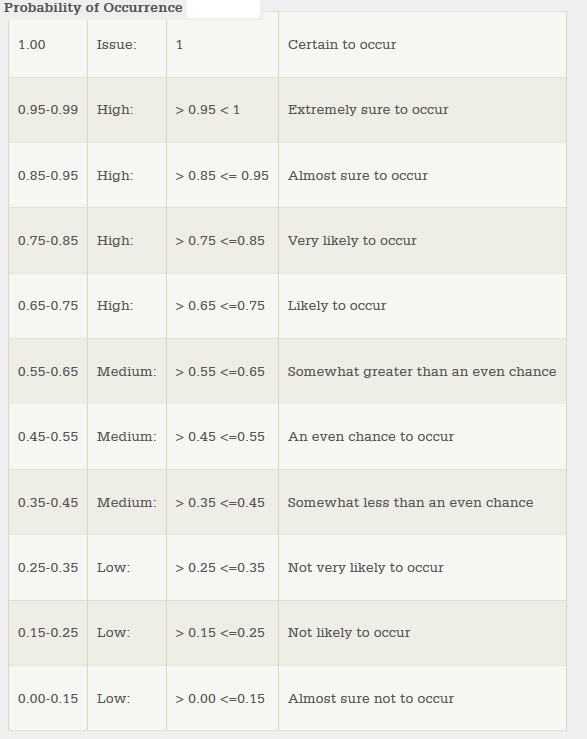
\includegraphics[scale=0.5]{3-requirements/Images/RISKSOCCURENCE.jpg} % maybe in the appendice ?
\subsection{Technical}

\risk{T}
{The warning system does not detect floods in time}
{Low}
{Severe because of the loss of human lives and money (estimate how much ?),loss of credibility regarding the end-users.}
{Make sure the number of sensors is sufficient and that they are in good state (as low failure rate as possible : repair or replace them ) thanks to a weekly checking for example.}
{ }
~\\[0.1cm]

\risk{T}
{The system sends warnings of a non-existing flood (false positive)} % WHEN THERE IS A FLOOD YOU KNOW IT
{Low}
{Moderate. People become more negligent to future messages.}
{UAV's watching the area where the supposed flood is. Hiring an operator to control}
{Send a message as soon as the mistake is detected to tell the population it was a false alert. }

\risk{T}
{The system can't send messages to the necessary people because the communication platform is also destroyed by the flood.}
{Medium}
{Severe . Loss of human lives and money }
{Find another way to get the phone number of a population}
{Using other medias : television, radio, Internet , ... }
	
\risk{T}
{The system sends incorrect information, causing extra damage.}
{Low}
{High . Loss of money and maybe lives.}
{Operator checking the validity of the information sent by the system.
	Good collaboration with the insurance companies.}
{  }

\risk{T}
{Hacker gets access to the system}
{Low}
{High. The hackers may sent incorrect information deliberately during the flood : Loss of money and maybe human lives. The system isn't reliable anymore.}
{Change password and hash codes every three months. Hire specialists in the security field.}
{Update the security system / change it. Find a new algorithm for the creation of password and hash codes.}



\subsection{Business}

\risk{B}
{Wrong estimation of the budget}
{Medium}
{High . The final product hasn't the features expected.}
{The team needs an accountant or at least someone taking care of the follow-up of the money.}
{Remove some requirements or features of the product.}

\risk{B}
{The money invested in the fabrication and achievement of the product/system is not covered by the sales (shortfall/deficit)}
{Medium}
{High. Stopping the sale}
{The team needs an accountant or at least someone taking care of the follow-up of the money.}
{Adding more features to the product in order to make it more competitive in the market.}

\risk{B}
{Competitors lowering their prices}
{Medium}
{Moderate. Loss of money.}
{  }
{  }
	
	
	%\textbf{ B-RISK4 The sensors company become bankrupt or at least stops its sales.} \\
	%\textit{Probability of Occurence}: Low \\
	%\textit{Consequences}: High.\\
	%\textit{Prevention} Our system use sensors from different companies \\
	%\textit{Decision}: Find another company selling sensors and make sure of its reliability. \\


\subsection{Schedule}
\risk{S}
{The project is not finished at the deadline}
{Low}
{Pressure for all the team members, loss of credibility regarding the end-users, selling a product with less features than expected.}
{ Meeting for the team members every week to keep track of the timing and take decisions according to the deadline. }
{ Remove some requirements or features in order to finish the project as soon as possible. }